\chapter{Abstract Algebra Basics}

What does ``abstract'' mean in the context of abstract algebra? How is abstract algebra different from classic algebra that has been introduced in earlier chapters? In short, classic algebra solves a particular problem using algebra algorithms, whereas abstract algebra studies these algorithms.

As an example, consider the following equation
\begin{eqnarray}
  Ax &=& y \nonumber
\end{eqnarray}
where $x$, $y$ are vectors and $A$ a matrix. Solving $x$ given particular $A$ and $y$ falls into the classic algebra domain. It is obvious that $x$ does not necessarily exist or being unique for different $y$ and $A$. Studying the general rules when $x$ exists and when it is unique for a set of $y$ and $A$ becomes an abstract algebra problem.

Consider another example where
\begin{eqnarray}
 a+b &=& b+a \nonumber \\
  ab &=& ba \nonumber
\end{eqnarray}
which are often used to demonstrate the commutative property of calculations (summation and multiplication, in this example). In classic algebra, they are considered as ground truth. In abstract algebra, however, the focus shifts to a more formal and generalized understanding of the property. We need to dig deeper into how commutative property is defined, and why it holds true for summation and multiplication, but not for some other operations such as division.

In conclusion, while classic algebra performs calculations on numbers, vector and matrices, abstract algebra studies the concepts, tools, derivations and logic we use in the calculation, and tries to explain why they work in the way they do. Abstract algebra also develops new concepts, tools and algorithms that we can use to solve more complicated algebraic problems.

\section{A Motivating Example}

One of the most famous applications of abstract algebra is to study the analytical solution to the following polynomial equation
\begin{eqnarray}
  x^n + a_1x^{n-1} + a_2x^{n-2} + \ldots + a_n &=& 0 \label{eq:polynomial_equation}
\end{eqnarray}
where $n\geq 1$ is the order of the polynomial and $a_1, \ldots, a_n$ are any arbitrary values. The analytical solutions to \eqref{eq:polynomial_equation} for $n=1$ and $n=2$ are obvious. With some effort, the analytical solutions for $n=3$ and $n=4$ were found in the $16$th century. Since then, people have been struggling to find the analytical solution to the fifth order and beyond $n\geq5$ polynomial equations.

In the $18$th and $19$th century, Euler, Lagrange and Gaussian tried to address this problem. Their conclusion was that there is no analytical solution to polynomial equations of fifth order or higher, but they could not give a very solid proof to the statement. Nevertheless, the methods they used inspired a lot of people that would work on this problem.

In the $19$th century, Abel was able to prove that there is no solution in radicals to general polynomial equations of fifth degree or higher with arbitrary coefficients (see Abel–Ruffini theorem). Furthermore, he discussed a set of special cases (with non-arbitrary coefficients in the polynomial equation) that can have analytical solutions. These special cases form a set of sufficient condition for a fifth order polynomial equation to have the analytical solution. 

The necessary and sufficient condition for a fifth or higher order polynomial to have an analytical solution is finally fully discovered by the genius Galois at a remarkably young age. Galois was able to create his theorem (known Galois theorem) and use it to find the ultimate answer to this problem that people have been studied for centuries. His theorem goes far beyond that. Galois theorem will find its usefulness in many areas to come, and eventually it becomes an important building block of a subject known as abstract algebra today. 

\section{General Algebraic System}

An algebraic system is essentially a mathematical system consisting of a non-empty set known as the domain together with a series of operations defined on the domain. There are many algebraic systems, and abstract algebra studies the properties of different algebraic systems. As will be introduced in later parts of the notebook, depending on the properties of the algebraic system, we can categorize them as groups, rings, fields, vector spaces, etc.

\subsection{Set and Mapping}

Set is one of the most commonly used terms across different mathematical subjects. It is also one of the fundamental concepts in abstract algebra. A set usually refers to a collection of distinct objects. Given a set $U$ and an object $x$, one and only one of the following two statements must be true:
\begin{itemize}
  \item Object $x$ is a member of set $U$, denoted by $x \in U$;
  \item Object $x$ is not a member of set $U$, denoted by $x \notin U$.
\end{itemize}
However, notice that due to the Russell's paradox, it is challenging to give a rigorous mathematical definition to a set that fulfill the above features.

Mapping, or function, is used to describe the association of elements in two sets. Mapping and function are used interchangeably in the this notebook. For example, let $A$ be a set, and $A_0 \subset A$ a subset of $A$. For any element $x\in A_0$, define mapping
\begin{eqnarray}
  i &:& A_0 \rightarrow A \nonumber
\end{eqnarray}
where
\begin{eqnarray}
  i(x) &=& x \nonumber
\end{eqnarray}
In this case, mapping $i$ is called the \textbf{embedding mapping} from $A_0$ to $A$.

Let $A$, $B$ be two sets, and $A_0 \subset A$ as subset of $A$. Let $f: A\rightarrow B$, and $g: A_0\rightarrow B$. Let $x\in A_0$. If $f(x)=g(x)$, function $f$ is known as an \textbf{extension} of function $g$, and function $g$ a \textbf{restriction} of function $f$ (on $A_0$). This is denoted by $g=f|_{A_0}$.

Mappings can be chained together. For example, consider two mappings
\begin{eqnarray}
	f_1 &:& A_1 \rightarrow A_2 \nonumber \\
	f_2 &:& A_2 \rightarrow A_3 \nonumber \\
	f_3 &:& A_3 \rightarrow A_4 \nonumber
\end{eqnarray}
With the above, we can denote $f = f_3\circ f_2\circ f_1$ a mapping from $A_1$ to $A_4$. Meantime, consider other mappings
\begin{eqnarray}
	g_1 &:& A_1 \rightarrow B \nonumber \\
	g_2 &:& B \rightarrow A_4 \nonumber 
\end{eqnarray}
Clearly, $g = g_2\circ g_1$ is also a mapping from $A_1$ to $A_4$. The mappings above can be illustrated intuitively using the \textbf{mapping diagram} in Fig. \ref{fig:mapping_plot}.
\begin{figure}[htbp]
	\centering
	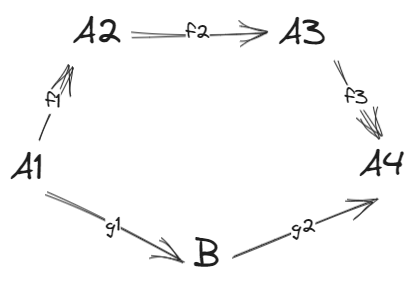
\includegraphics[width=200pt]{chapters/abstract-algebra-basics/figures/mapping_plot.png}
	\caption{Mapping diagram that demonstrates $f$ and $g$.} \label{fig:mapping_plot}
\end{figure}
Mapping diagram can become handy with some complicated mappings.

The embedding mapping, extension function and restriction function introduced earlier can also be represented by a mapping diagram as shown in Fig. \ref{fig:embedding_mapping_plot}, where $A_0 \subset A$ and $i:A_0\rightarrow A$ a embedding mapping. Function $g$ defined on the subset $A_0$ is a restriction of $f$ defined on the superset, whereas $f$ is an extension of $g$, i.e., $f(x) = g(x)$ for $x\in A_0$.
\begin{figure}[htbp]
	\centering
	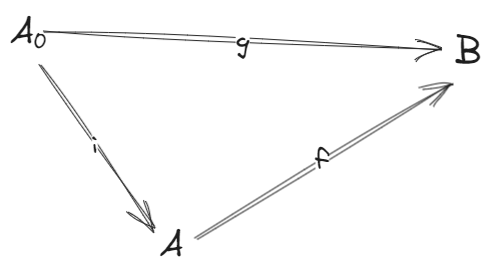
\includegraphics[width=200pt]{chapters/abstract-algebra-basics/figures/embedding_mapping_plot.png}
	\caption{Mapping diagram of embedding mapping.} \label{fig:embedding_mapping_plot}
\end{figure}

Multiple sets can be ``combined'' and ``augmented'' to form new sets. For example, the \textbf{Cartesian product} of two sets, $A_1$ and $A_2$, is defined as follows.
\begin{eqnarray}
	A_1 \times A_2 = \left\{(a,b) \middle| a \in A_1, b\in A_2\right\} \nonumber
\end{eqnarray}
where the tuple $(a,b)$ can be interpreted as a probable ordered combination of elements in $A_1$ and $A_2$. The idea can be applied similarly to more sets.

\subsection{Operation}

Summation, multiplication, etc., are operations. In abstract algebra, we are more interested in the broad definition of operations from set perspective, instead of listing down individual operations and study how they work.

An operation essentially describes the rule of deriving or mapping from one or multiple elements to a new element, each element belongs to some non-empty set. Take binary operation as an example which maps two elements to one element. Let $A$, $B$, $D$ be three non-empty sets. Let $f$ be a mapping
\begin{eqnarray}
	f &:& A \times B \rightarrow D \label{eq:operation_general_def}
\end{eqnarray}
Then $f$ is called a algebraic operation from $A$, $B$ to $D$. The operation can be denoted by $f(a,b)$ where $a\in A$ and $b\in B$. For convenience, binary operation is often denoted by $a\oplus b$, $a\otimes b$, or something similar from the writer preference. Notice that there are conventions to follow when using the symbols. For example, $+$, $-$, $\times$, etc., already have clear meanings.

The following is an example of operations. Let the domain of interest be $\mathbb{R}$, which is the real number set. Let $v$ be a vector space (a set that contains a bunch of vectors) defined under $\mathbb{R}^n$. We can then define summation $+$ as a binary operation
\begin{eqnarray}
	+ &:& v\times v \rightarrow v \nonumber
\end{eqnarray} 
which indicates that the summation takes in two elements in the vector space, and generates a new vector that also belongs to the same vector space. 

In the case where the domain and range of the operation come from the same set, i.e., in \eqref{eq:operation_general_def} $A=B=D$, the operation is said to be \textbf{closed} under this operation. In this example, the summation operation $+$ defined on $v$ is closed, and we can simply say ``$+$ is a binary operation defined on $v$''.

Operations may have some unique properties. For example, let binary operation defined on $A$, denoted by $\oplus $, i.e., $\oplus: A\times A \rightarrow A$. If
\begin{eqnarray}
	a \oplus b &=& b \oplus a, \forall a, b \in A \nonumber
\end{eqnarray}
then the operation is said to have \textbf{commutative property}. If
\begin{eqnarray}
	a \oplus (b \oplus c) &=& (a \oplus b) \oplus c, \forall a,b,c \in A \label{eq:associative_property}
\end{eqnarray}
then the operation is said to have \textbf{associative property}, and \eqref{eq:associative_property} can be simply denoted by $a \oplus b \oplus c$. Let two binary operations defined on $A$, denoted by $\oplus$ and $\otimes$ respectively. If
\begin{eqnarray}
	a \oplus (b \otimes c) &=& (a \oplus b) \otimes (a \oplus c) \nonumber
\end{eqnarray}
then the operation $\oplus$ is said to have the left-hand \textbf{distributive property} on operation $\otimes$. Similarly, right-hand distributive property can also be defined.  

Commutative property, associative property and distributive property are commonly seen and widely discussed properties of operations. When operations have some of the three properties, simplified notation may apply. For example, if $\oplus$ operation has associative property, then
\begin{eqnarray}
	a^n &\equiv& \overbrace{a \oplus \cdots \oplus a}^{n} \nonumber
\end{eqnarray}
can be used. If both commutative and associative properties hold, then it can be easily proved that
\begin{eqnarray}
	a^nb^n & = & (ab)^n \nonumber 
\end{eqnarray}

There are several different ways to present the result of an operation. When the cardinal number of the input sets are finite, a simple way is to list all the input-output associations in a table. An example is given in Fig. \ref{fig:logical_and_mapping} which exhaustively lists down ``and'' logical operation results.
\begin{figure}[htbp]
	\centering
	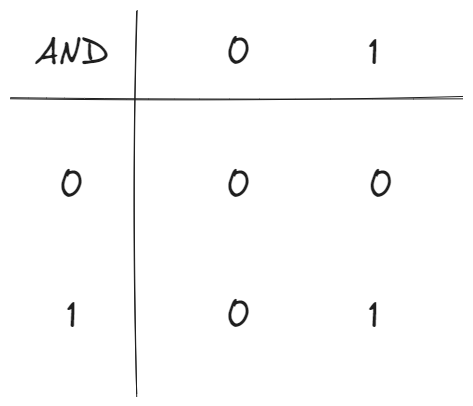
\includegraphics[width=150pt]{chapters/abstract-algebra-basics/figures/logical_and_mapping.png}
	\caption{Result of ``and'' logical operation.} \label{fig:logical_and_mapping}
\end{figure}

\subsection{Relation}

Consider the relation of two elements $a$ and $b$. In mathematics, relation essentially describes a property that the tuple made from the two elements, i.e. $(a,b)$, may or may not have. Therefore, a straight forward way of defining a relation is to construct a set that contains some tuples, and if the specified tuple $(a,b)$ is in the set, we say $a$, $b$ have that relation, and equivalently $(a,b)$ has that associated property.

For example, consider $a,b\in\mathbb{Z}$. Define relation
\begin{eqnarray}
	R = \left\{(a,b)~\middle|~a-b = kn,~k,n \in\mathbb{Z}, n>1\right\}
\end{eqnarray}
where $\mathbb{Z}$ denotes the integer set. If $a$, $b$ are such that $(a,b)\in R$, we say $a$, $b$ are congruent modulo $n$, which is a congruence relation and can be denoted by
\begin{eqnarray}
	a &\equiv& b~(\textup{mod}~n) \nonumber
\end{eqnarray}

To summarize, let $a\in A$, $b\in B$. Let $R\subset A\times B$ be a subset of $A\times B$. the following statements can be considered equivalent:
\begin{itemize}
	\item Two elements $a$ and $b$ have relation $R$;
	\item Tuple $(a,b)$ has the property associated with relation $R$;
	\item Tuple $(a,b) \in R$;
\end{itemize}
and in that case we can use $aRb$ to signify the relation. From above, we can see that each relation is associated with a subset $R$ defined on the Cartesian product of the sets that the two elements belong to, and vise versa.

Like the case of operation where commutative, associative and distributive properties are defined, relation can also have special properties. For example, let relation $R$ be defined on $A \times A$. If $\forall a,b,c \in A$,
\begin{eqnarray}
	aRa \nonumber
\end{eqnarray}
then $R$ is said to be \textbf{reflexive}. If
\begin{eqnarray}
	aRb &\Rightarrow& bRa \nonumber
\end{eqnarray}
then $R$ is said to be \textbf{symmetric}. If
\begin{eqnarray}
	aRb, bRc &\Rightarrow& aRc \nonumber 
\end{eqnarray}
then $R$ is said to be \textbf{transitive}. Finally, if
\begin{eqnarray}
	aRb, bRa &\Rightarrow& a=b \nonumber 
\end{eqnarray}
then $R$ is said to be \textbf{antisymmetric}.

From the above definitions, we can see that the commonly seen ``$=$'' relation defined on $\mathbb{R}\times\mathbb{R}$ is reflexive, symmetric and transitive. Similarly, ``$\leq$'' is reflexive, transitive and antisymmetric.

If a relation is simultaneously reflexive, symmetric and transitive, it is called an \textbf{equivalence relation}. The equal ``$=$'' relation and congruence relation introduced earlier are examples of equivalence relation.

We can define a \textbf{partition of a (non-empty) set} by grouping its elements into non-empty subsets in such a way that every element is included in exactly one subset, i.e.
\begin{eqnarray}
	A &=& \bigcup_{i\in I}A_i, \forall i, j \in I, i\neq j, A_i \neq \varnothing, A_i \bigcap A_j = \varnothing \nonumber
\end{eqnarray}
A partition of a set can form a new set $\{A_i\}$. Furthermore, we can define a relation $R\subset A \times A$ on top of that partition as follows
\begin{eqnarray}
	R = \left\{(a,b)~\middle|~\exists i, a,b \in A_i\right\} \nonumber
\end{eqnarray}
and it is clear that such $R$ is an equivalence relation. A partition of a set $A$ can determine an equivalence relation $R\subset A\times A$ using the above method. Vise versa, an equivalence relation $R\subset A\times A$ can also determine a partition of set $A$ as follows. For $\forall a \in A$, define
\begin{eqnarray}
	[a] &=& \left\{b \in A\middle| aRb \right\} \nonumber
\end{eqnarray}
where $R$ is the equivalence relation, and $[a]$ the \textbf{equivalence class} of $a$. 

With the definition of equivalence class, a partition of a set $A$ can then derived from the equivalence relation $R$ by
\begin{eqnarray}
	A/R &=& \left\{[a] | a \in A \right\} \textup{(remove duplication)} \label{eq:quotient_set}
\end{eqnarray}
where $A/R$ is the partition of set $A$ (this can be proved easily) derived from equivalence relation $R$. Notice that $[a]$ derived from different $a$ yet in the same equivalence class will duplicate. When putting duplicated $[a]$ into a set, duplication should be removed, hence the note ``remove duplication''. It is not compulsory to add that note because it is inherently addressed by the fundamental properties of a set. The partition of set obtained using the above method is known as the \textbf{quotient set}. There is a one-to-one correspondence between an equivalent relation a partition of the set which is also known as the quotient set of that corresponding equivalent relation.

Given an equivalence relation, the following mappings can be defined.
\begin{eqnarray}
	\pi &:& A \rightarrow A/R, ~\pi(a) = [a] \nonumber
\end{eqnarray}
which is known as the \textbf{canonical projection} or \textbf{quotient map}.

\subsection{Congruent Modulo}

We have introduced congruent modulo in the context of number theory as an example of equivalence relation. In that example, when two integers $a$ and $b$ are congruent modulo $n$, their equivalence relation persists even if $k_1n$, $k_2n$ are added or subtracted from both of them respectively.

The concept of congruent modulo can be further generalized in the context of operation and equivalence relation as follows. Let $A$ be an non-empty set. Let $\oplus$ be a closed binary operation defined on $A$, i.e., $\oplus: A\times A \rightarrow A$. Let $R$ be an equivalence relation defined on $A$, i.e., $R\subset A\times A$, and $A/R$ its corresponding quotient set. Let $a_1, a_2, b_1, b_2 \in A$. If operation $\oplus$ and equivalence relation $R$ satisfy the following condition
\begin{eqnarray}
	a_1Ra_2, ~b_1Rb_2 &\Rightarrow& (a_1\oplus b_1)R(a_2\oplus b_2) \label{eq:relation_congruent_modulo_operation}
\end{eqnarray}
then we say that $R$ is congruent modulo $\oplus$. This is demonstrated by Fig. \ref{fig:congruent_modulo_relation} the left plot.
\begin{figure}[htbp]
	\centering
	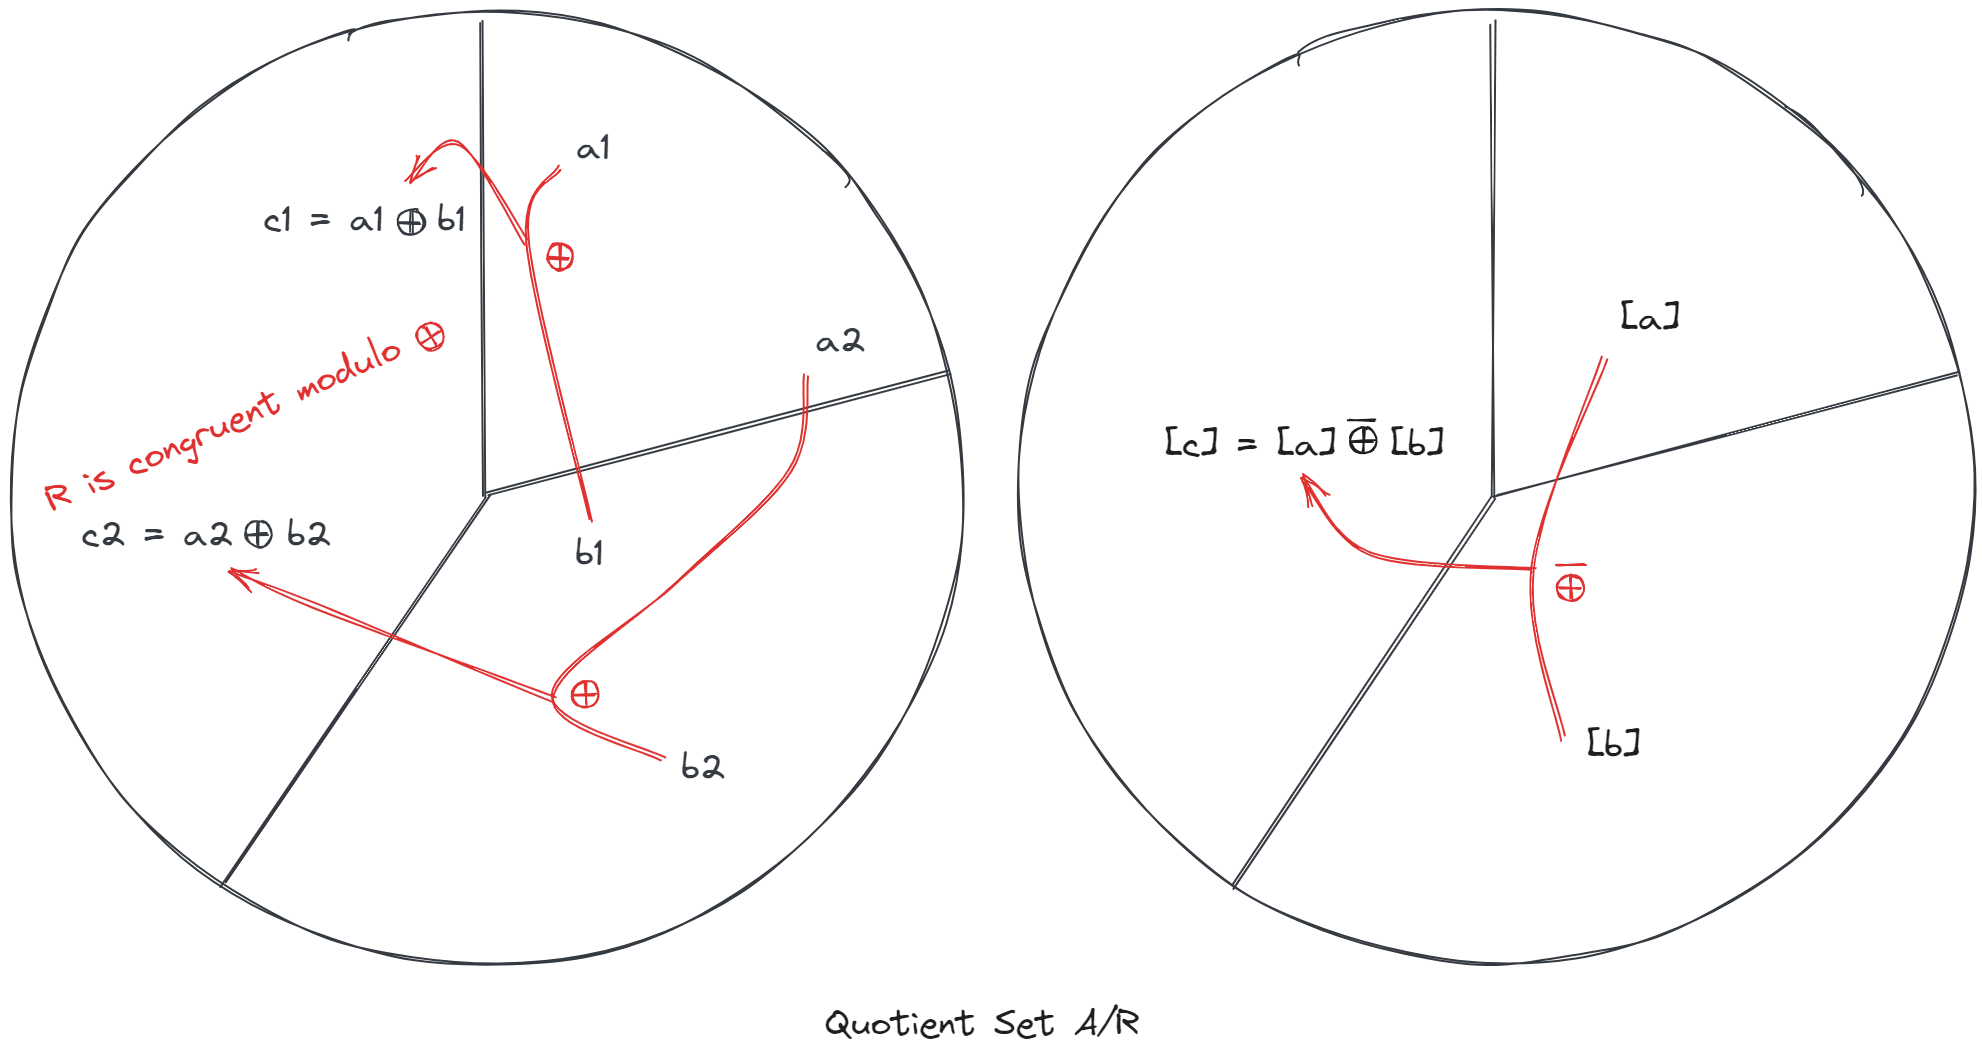
\includegraphics[width=350pt]{chapters/abstract-algebra-basics/figures/congruent_modulo_relation.png}
	\caption{A relation is congruent modulo an operation.} \label{fig:congruent_modulo_relation}
\end{figure}
From Fig. \ref{fig:congruent_modulo_relation} the left plot, it can be intuitively interpreted that when two elements $a_1$, $b_1$ are equivalent, their equivalence relation persists even if operation $\oplus a_2$, $\oplus b_2$ are applied to them respectively, so long as $a_2$, $b_2$ are also equivalent.

If $R$ is congruent modulo $\oplus$ indeed, we can define an operation on the quotient set $A/R$ as follows. Let $[\cdot]$ denote the equivalence class of an element in $A$. Define $\bar{\oplus}$ as an operation on $A/R$ as follows.
\begin{eqnarray}
	[a] \bar{\oplus} [b] &=& [a\oplus b], ~a\in[a], ~b\in [b] \label{eq:quotient_set_operation}
\end{eqnarray}
where $a$, $b$ are arbitrarily selected elements in the equivalence class $[a]$ and $[b]$ respectively, as shown in Fig. \ref{fig:congruent_modulo_relation} right plot. Notice that $[a\oplus b]$ should be well-defined regardless of the choice of $a$ and $b$ so long as they are selected in their associated equivalence class $[a]$ and $[b]$ respectively since $R$ is congruent modulo $\oplus$. In this context, $\bar{\oplus}$ is known as the \textbf{included operation} or \textbf{quotient operation} of $\oplus$ on the quotient set $A/R$.

To conclude, in the algebraic system with non-empty set $A$ and an operation $\oplus$ (denoted by $\{A; \oplus\}$), if there is a equivalent relation $R$ which is congruent modulo $\oplus$, we can construct a new algebraic system $\{A/R; \bar{\oplus}\}$, where $A/R$ is the quotient set of $A$ on $R$ from \eqref{eq:quotient_set}, and $\bar{\oplus}$ the included operation of $\oplus$ on $A/R$ from \eqref{eq:quotient_set_operation}.

\section{Semi-Group and Group}

In the previous section, general algebraic system is introduced. A general algebraic system shall contain a set of interest as well as one or more operation defined on that set. The operations can be unary (involving one operand), binary (involving two operands), ternary (involving three operands), etc. Relations within these systems are defined as sets of tuples, with each element of the tuple coming from the set of interest. Likewise, relation can also be binary, ternary, etc.

Special properties can apply to both operations and relations. Binary operations, for instance, can exhibit commutativity, associativity, and distributivity. Binary relations, on the other hand, can be reflexive, symmetric, and transitive.  If a relation is simultaneously reflexive, symmetric and transitive, it is called a equivalent relation. Each equivalent relation is corresponded with a quotient set which is a partition of the original set by equivalence classes of the relation.

When a relation is congruent modulo an operation (recall \eqref{eq:relation_congruent_modulo_operation} and Fig. \ref{fig:congruent_modulo_relation}), we can establish a new algebraic system. This system comprises the quotient set and a well-defined induced operation on that set. The new system retains structural properties from the original set, reflecting the consistency and compatibility of the congruence relation with the operation.

Moving forward, our focus will shift to specialized algebraic systems characterized by distinctive properties. This exploration will pave the way to understanding the fundamental algebraic structures such as semi-groups, groups, and rings. We will see the critical impact the operation possess over the algebraic system. Even with the same set, different operations often leads to very different features of the algebraic system.

\subsection{Semi-Group}

Let $S$ be a non-empty set, and $\oplus: S\times S \rightarrow S$ a closed binary operation defined on $S$. If $\oplus$ has associative property, i.e. $a\oplus(b\oplus c) = (a \oplus b) \oplus c$, then algebraic system $\{S; \oplus\}$ (for simplicity, $S$, when there is no ambiguity) is called a \textbf{semi-group}.

Examples of semi-group include $\{\mathbb{N}; +\}$, $\{\mathbb{N}; \times\}$ where $\mathbb{N}$ refers to the (positive) natural numbers $1, 2, 3, \ldots$. Let $A$ be an non-empty set, and $\{\mathcal{M}(A); \circ\}$ is also a semi-group, where $\mathcal{M}(A)$ is the set of all the closed mappings defined on $A$, and $\circ$ the compound operation. Additionally, $\{\mathcal{P}(A); \bigcup\}$, $\{\mathcal{P}(A); \bigcap\}$ are also semi-groups, where $\mathcal{P}(A)$ represents the power set of $A$.

\begin{shortbox}
\Boxhead{Is Zero Included in Natural Numbers?}
The definition of natural numbers may or may not include zero ``$0$'' depending on the context. In the context of number theory and abstract algebra, natural numbers often exclude zero.
\end{shortbox}

\subsection{Monoid}

Consider semi-group $\{S; \oplus\}$. If $\exists e\in S$ so that
\begin{eqnarray}
	e\oplus a &=& a, ~\forall a \in S \nonumber
\end{eqnarray}
then $e_1$ is known as the \textbf{left identity}. Similarly, we can define \textbf{right identity}. Notice that a semi-group may have many distinct left and right identities.

If an element $e$ is both left identity and right identity, it is called the \textbf{identity element}. If a semi-group has an identity element, the identity element must be unique. This can be easily illustrated using proof by contradiction as follows. Assume that $e_1$, $e_2$ are two distinct identity elements, thus
\begin{eqnarray}
	e_1\oplus e_2 = e_1 &\textup{and}& e_1\oplus e_2 = e_2 \nonumber
\end{eqnarray}
indicating $e_1=e_2$, which contradicts with the assumption.

A semi-group with the identity element is knows as a \textbf{monoid}. From the definition, we know that $\{\mathbb{N}; \times\}$, $\{\mathcal{M}(A); \circ\}$, $\{\mathcal{P}(A); \bigcup\}$ and $\{\mathcal{P}(A); \bigcap\}$ are all monoids, with their identity elements being $1$, $f: A\rightarrow A, f(a)=a$, $\varnothing$ and $A$, respectively.

\subsection{Group}

Let $\{S; \oplus\}$ be a monoid with identity element $e$. If for $a\in S$, there is
\begin{eqnarray}
	a\textprime \oplus a &=& e \nonumber
\end{eqnarray}
then $a\textprime$ is called the left inverse of $a$. Likewise, right inverse can be defined. Notice that an element may have many left and right inverses.

If $a\textprime$ is both the left and the right inverse of $a$, then $a\textprime$ is known as the inverse of $a$. In this case, similar to the identity element, $a\textprime$ must be unique. The proof can be obtained similarly using proof by contradiction. The inverse of $a$ is often denoted by $a^{-1}$.

If in a monoid $\{S; \oplus\}$, there is the inverse for all its elements, the monoid is called a group, usually denoted by $\{G; \oplus\}$, or simply $G$ when without ambiguity.

The relationship of general algebraic system, semi-group, monoid and group are demonstrated in Fig. \ref{fig:group_definition}.
\begin{figure}[htbp]
	\centering
	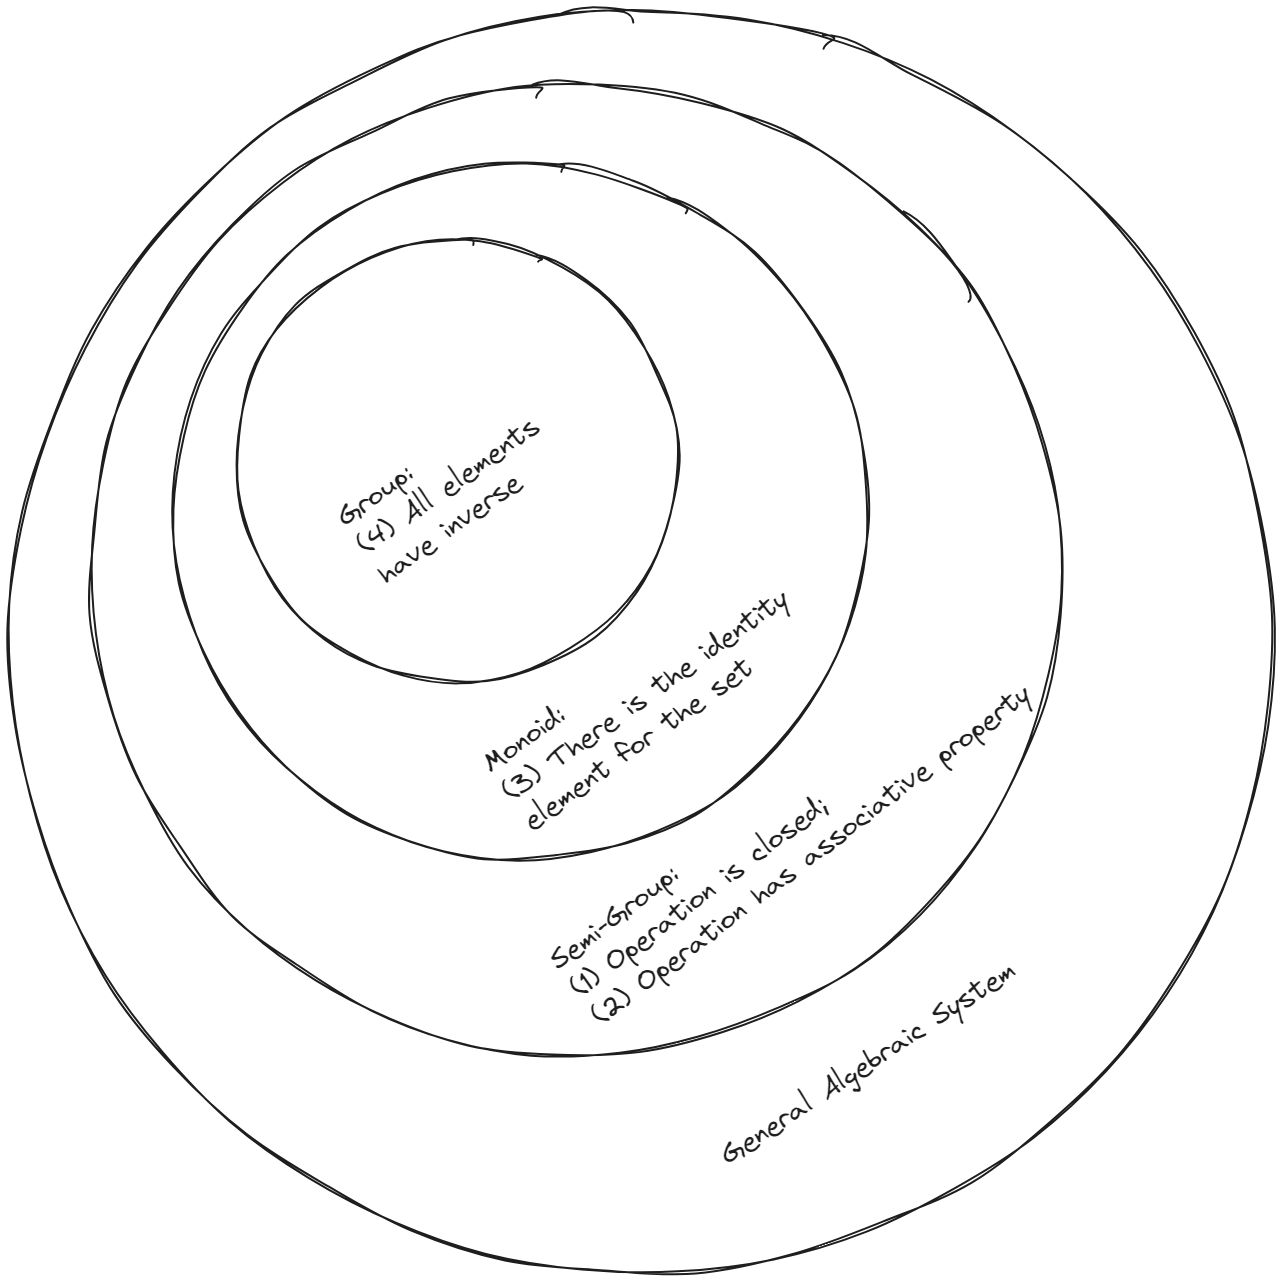
\includegraphics[width=300pt]{chapters/abstract-algebra-basics/figures/group_definition.png}
	\caption{General Algebraic System, Semi-Group, Monoid and Group.} \label{fig:group_definition}
\end{figure}

Notice that group does not pre-assume commutativity. If a group's operation is commutative, it is called an \textbf{abelian group} named after Niels Henrik Abel. Examples of abelian group include $\{\mathbb{Z}; +\}$, $\{\mathbb{R}; +\}$, $\{\mathbb{C}; +\}$ where $\mathbb{Z}$, $\mathbb{R}$ and $\mathbb{C}$ represent integer set, real number set and complex number set, respectively. Additionally, $\{\mathbb{R}^{*}; \times \}$, $\{\mathbb{R}^{*}; \times \}$ are also abelian groups, where $\mathbb{R}^*$,  $\mathbb{C}^*$ denotes the corresponding sets excluding zero.

We know that $\{\mathcal{M}(A); \circ\}$ introduced earlier is not a group. This is because not all mappings defined on a set $A$ necessarily have an inverse. However, if define $\{\mathcal{S}(A); \circ\}$ where $\mathcal{S}(A)$ represents the set of all  bijections (invertible mappings) on $A$, $\{\mathcal{S}(A); \circ\}$ becomes a group. Notice that $\mathcal{S}(A)$ is not necessarily an abelian group.

To conclude, a group must meet the following requirement:
\begin{itemize}
	\item There is a non-empty set $G$;
	\item There is a closed binary operation $\oplus: G\times G \rightarrow G$;
	\item The operation $\oplus$ has associative property, i.e. $\forall a, b, c \in G, (a \oplus b) \oplus c = a\oplus (b \oplus c)$;
	\item There is the identity element, i.e. $\exists e\in G$, $\forall a \in G, e\oplus a = a \oplus e = a$;
	\item There is the inverse for all elements, i.e., $\forall a\in G$, $\exists a^{-1}$, $a\oplus a^{-1} = a^{-1}\oplus a = e$;
\end{itemize}
Furthermore, if
\begin{itemize}
	\item Operation $\oplus$ has commutative property, i.e. $\forall a, b\in G, a\oplus b=b\oplus a$;
\end{itemize}
the group is called an abelian group.

It can be proved that if a semi-group has left identity and all its elements have left inverse, the left identity must also be its right identity and all its elements must also have left reverse, thus making the semi-group a group. The proof is given below. Let $e$ be the left identity of semi-group $\{S;\oplus \}$, while $b$ be the left inverse of any arbitrary element $a\in S$. Let $c$ be the left inverse of $b$.
\begin{eqnarray}
a\oplus b &=& e\oplus a\oplus b \nonumber \\
   &=& c\oplus (b\oplus a)\oplus b ~\textup{(associativity)} \nonumber \\
   &=& c\oplus (e\oplus b) ~\textup{(associativity)} \nonumber \\ 
   &=& c\oplus b \nonumber \\ 
   &=& e \nonumber
\end{eqnarray}
Therefore, $b$ is also the right inverse of $a$. Furthermore,
\begin{eqnarray}
a\oplus e &=& (a\oplus b)\oplus a ~\textup{(associativity)} \nonumber \\
   &=& e\oplus a \nonumber \\
   &=& a \nonumber
\end{eqnarray}
Therefore, $e$ is also the right identity. All the above derivations also apply when a semi-group has right identity and all its elements have right inverse.

\subsection{Properties of Semi-group and Group}

Commonly used properties and notations of semi-group and group are introduced in this section.

If $S$ is a semi-group and $a, b \in S$, then the following criteria can be used to further determine that $S$ is a group.
\begin{itemize}
  \item For $\forall a, b \in S$, if both $ax = b$ and $xa = b$ have solution, then $S$ is a group.
  \item If $|S|<\infty$ (cardinal number of $S$ is finite), and $\forall a, b, c \in S$, $ac = bc \Rightarrow a = b$, $ca = cb \Rightarrow a = b$, then $S$ is a group.
\end{itemize}

If $G$ is a group and $a, b, c \in G$, then the following properties apply. 
\begin{itemize}
  \item $ac = bc \Rightarrow a = b$;
  \item $ca = cb \Rightarrow a = b$;
  \item $ax = b$ has the unique solution $x = a^{-1}b$; $xa = b$ has the unique solution $x = ba^{-1}$;
\end{itemize}

Given group $\{G;\oplus\}$ and $a\in G$. The following notations apply.
\begin{eqnarray}
  a^n &\equiv&  \overbrace{a \oplus \cdots \oplus a}^{n} \label{eq:group_exponential_1} \\
  a^0 &\equiv& e \label{eq:group_exponential_2} \\
  a^{-n} &\equiv& \overbrace{a^{-1} \oplus \cdots \oplus a^{-1}}^{n} \label{eq:group_exponential_3}
\end{eqnarray}
where $n$ is a positive integer, $e$ the identity element of $G$ and $a^{-1}$ the inverse of $a$. With this notation, instead of \eqref{eq:group_exponential_1}, \eqref{eq:group_exponential_2} and \eqref{eq:group_exponential_3}, the following properties apply.
\begin{itemize}
  \item $a^ma^n = a^{m+n}$
  \item $\left(a^m\right)^n = a^{mn}$
\end{itemize}

When studying abelian groups, ``$+$'' is most commonly used to represent the operation, and the following notations apply.
\begin{eqnarray}
  na &\equiv& \overbrace{a + \cdots + a}^{n} \nonumber \\
  0a &\equiv& e \label{eq:group_exponential_4} \\
  (-n)a &\equiv& \overbrace{(-a) + \cdots + (-a)}^{n} \nonumber
\end{eqnarray}
where $-a$ is used to denote the inverse of $a$. In this case, the identity element $e$ in \eqref{eq:group_exponential_4} is often denoted by ``$0$''. It might be confusing since it is visually the same with the numerical number zero, but what it really represents is the identity element of that group, not necessarily numerical zero. When the group $G$ is $\mathbb{Z}$, $\mathbb{R}$ or $\mathbb{C}$, and the operation is indeed summation, the identity element is indeed numerical zero.

The idea of group goes beyond number theory and mathematics. Generally speaking, any system that can move from states to states with movements revertible can be described by a group or something similar. When a system shows symmetry, it can probably be described by a group.

\subsection{Order of Elements in a Group}

Let $G$ be a group, $e$ its identity element, and $a\in G$. If there exists a smallest positive integer $n$ so that $a^n = e$, we say that the \textbf{order} of $a$ is $n$. If no such $n$ exists, the order of $a$ is infinity. The identity element $e$ is the only element that has an order of $1$. For an element with order $n$, its inverse also has the order of $n$.

Let $G$ be a group, $e$ its identity element, and $a\in G$. Consider the sequence of $a^n$ as follows.
\begin{eqnarray}
\begin{array}{ccccccccc}
  \ldots & a^{-3} & a^{-2} & a^{-1} & a^0 (e) & a^1 & a^2 & a^3 & \ldots \nonumber 
\end{array}
\end{eqnarray}
If $a$ has the order of infinity, then $a^m \neq a^n$ for any integers $m\neq n$, and vise versa. This can be easily proved with proof by contradiction. If an element has the order of $d$, then $a^m = a^n$ repeats if and only if $m-n = kd, k\in \mathbb{Z}$.

If $a \in G$ has order $d$, then $a^{k}, k\neq0$ has order $d/(d,|k|)$, where $(d,|k|)$ is the greatest common divisor of $d$ and $|k|$. This implies that $a^{k}$ has order no more than $d$, and it has order $d$ if and only if $(d,|k|)=1$.

If $a,b \in G$ has order $m$ and $n$ respectively, and $ab=ba$, then $ab$ and $ba$ have the order of $[m,n]$, where $[m,n]$ stands for the least common multiple of $m$ and $n$.

\section{Subgroup and Quotient Set}

Subgroup and quotient set are both fundamental concepts in group theory. They not only form an important part of abstract algebra by themselves, but also help with better understanding group and its properties.

\subsection{Subgroup}

Let $\{G;\oplus\}$ be a group, and $H\subset G, H\neq\varnothing$ is a non-empty subset of the group. If $\{H;\oplus\}$ forms a group under the same operation $\oplus$, then $H$ is called a \textbf{subgroup} of $G$, denoted by $H\leq G$. Notice that if $H \neq G$, $H$ is called a \textbf{proper subgroup} of $G$ and can be denoted by $H<G$. That implies that
\begin{itemize}
  \item The operation $\oplus$ which is close in $G$ is also close in $H$;
  \item The identity element of $G$, denoted by $e$, is in $H$;
  \item For every element $a\in H$, its inverse $a^{-1}$ is also in $H$.
\end{itemize}
Here is an example of a subgroup. Consider group $\{\mathbb{R}^*; \cdot\}$ where $\mathbb{R}^*$ denotes real number set excluding zero, and $\cdot$ the multiplication operation. Then group $\{\mathbb{R}^+;\cdot\}$ where $\mathbb{R}^+$ denoting positive real number set is a subgroup of  $\{\mathbb{R}^*; \cdot\}$.

The following criteria can be used to determine whether a subset is a subgroup under the operation. Let $\{G;\oplus\}$ be a group, and $H\subset G$ a non-empty subset. The following three statements are equivalent.
\begin{enumerate}[label=(\roman*)]
  \item $H\leq G$;
  \item $\forall a, b\in H$, $a\oplus b \in H$, $a^{-1}\in H$;
  \item $\forall a, b \in H$, $a\oplus b^{-1} \in H$.
\end{enumerate}
Furthermore, if $|H|<\infty$, the following two statements are equivalent.
\begin{enumerate}[label=(\roman*)]
  \item $H\leq G$;
  \item $\forall a, b\in H$, $a\oplus b \in H$.
\end{enumerate}
The proof is neglected in this notebook.


Subgroup has the following properties.  
\begin{itemize}
  \item If $H_1 < G$, $H_2 < G$, $H_1 \bigcap H_2 \neq \varnothing$, then $H_1 \bigcap H_2 < G$;
  \item If $H_1 < G$, $H_2 < G$, then $H_1 \bigcup H_2$ is not necessarily a subgroup of $G$.
\end{itemize}

\subsection{Coset}

Let $\{G;\oplus\}$ be a group, $H \leq G$ a subset, and $a\in G$. Define \textbf{left coset} $aH$ as follows.
\begin{eqnarray}
  aH &=& \left\{a\oplus h| h \in H \right\} \nonumber
\end{eqnarray} 
Similarly, the \textbf{right coset} $Ha$ can be defined.





























